\section{DHCP Setup}
This section describes how the \textbf{DHCP service} was set up in the \textit{Internal router} machine, the one reachable at address \textbf{100.100.2.1}.\\
The router was accessed via web browser in the \textbf{Kali machine} (\textbf{100.100.2.100} as static IP address) through the given credentials, and then the desired service was configured through the \textbf{OPNSense} administration panel.\\
The following steps were taken to give the service the proper configuration provided by the assignment:\\

\begin{itemize}
\item the service was enabled on the router, as pictured in \textbf{Figure 2}. Keep also in mind that the subnet mask was already specified in the \textbf{CLIENTS} interface for the router, and the same goes for other services - such as \textbf{Unbound DNS}, so that these settings were not required to be configured again;
\item the address range was initially specified as \textbf{100.100.2.101 - 100.100.2.253} so to avoid a re-assignment of known static IP addresses in the network - that is to say, those belonging to the Kali machine, the Arpwatch machine and, of course, the router itself. Later on, as pictured in \textbf{Figure 3}, a new pool of addresses was specified in the range \textbf{100.100.2.2 - 100.100.2.99} so to comprehend all the addresses that are not known to be assigned in the network;
\item as pictured in \textbf{Figure 4}, the partial \textbf{MAC addresses} pointed out in the assignment as allowed to make use of the service were specified in the configuration, so that the only machines able to receive DHCP offers from the router will be the ones exhibiting these MAC addresses;
\end{itemize}

\begin{figure}[htpb]
\centering
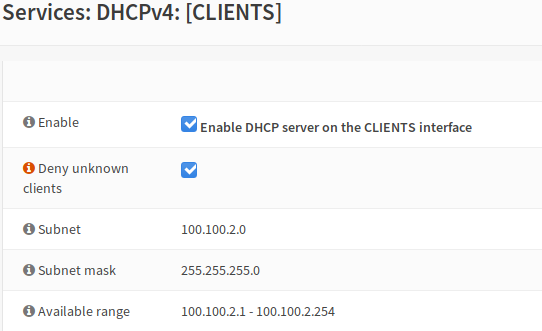
\includegraphics[width=0.5\textwidth]{dhcp_clients.png}
\caption[a]{Enabling the DHCP service on the Internal Router.}\label{fig:2}
\end{figure}

\begin{figure}[htpb]
\centering
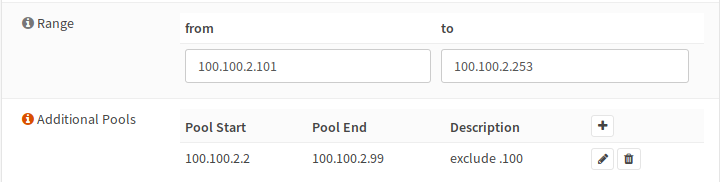
\includegraphics[width=0.7\textwidth]{dhcp_range.png}
\caption[a]{The specified range for assignable addresses on the DHCP service.}\label{fig:3}
\end{figure}

\begin{figure}[htpb]
\centering
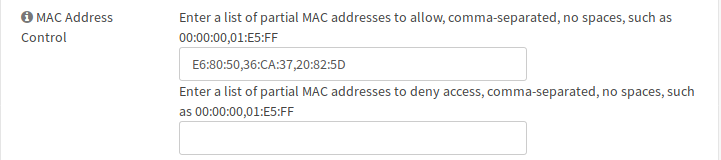
\includegraphics[width=0.7\textwidth]{dhcp_mac_rules.png}
\caption[a]{The partial MAC addresses specified in the configuration.}\label{fig:4}
\end{figure}

Once the \textbf{DHCP service} was confirmed running on the router, it was tested directly from the \textbf{Kali machine} by deleting the IP address set by default on \textbf{eth0} and thus trying to obtain a new one through the \textbf{DHCP service} of the router. First, as pictured in \textbf{Figure 5}, the \textbf{dhclient} command was run so that the machine could obtain a new dynamic IP address on the interface \textbf{eth0} - the machine has by default a \textbf{MAC address} on interface \textbf{eth0} which falls under the allowed addresses specified in the configuration. A \textbf{DHCP offer} was received by the router, and a new IP address was obtained, positively assessing the functioning of the service so far.\\
Again from the \textbf{Kali machine}, the \textbf{MAC address} of \textbf{eth0} was then changed to one that should not be allowed to request a new IP to the service, as pictured in \textbf{Figure 6}. The \textbf{dhclient} command was run again, and this time no offer was received, thus confirming that the service is only leasing IP addresses to machines having the desired \textbf{MAC addresses} on their interfaces.

\begin{figure}[htpb]
\centering
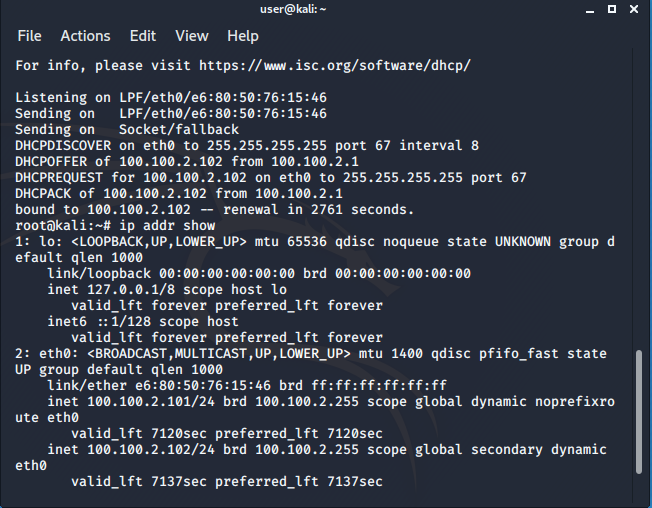
\includegraphics[width=0.7\textwidth]{dhcpoffer_received_kali.png}
\caption[a]{Kali machine with right MAC address on eth0 receiving a new IP address.}\label{fig:5}
\end{figure}

\begin{figure}[htpb]
\centering
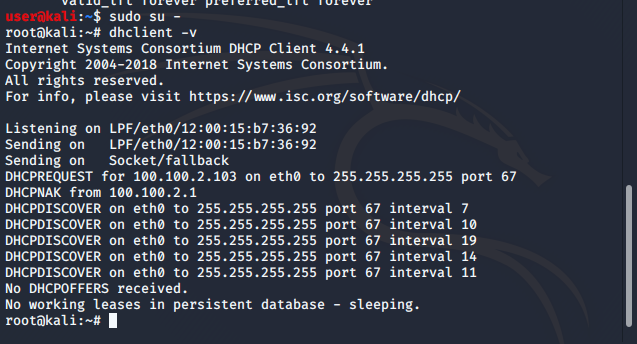
\includegraphics[width=0.7\textwidth]{dhcp_request_undesired_MAC_no_response.png}
\caption[a]{Kali machine unable to receive a DHCP offer due to its modified MAC address (not allowed).}\label{fig:6}
\end{figure}
